\subsection{Terrain Toolbox (Bogna Lew)}\label{ss:tTool}
Terrain Toolbox jest narzędziem dostępnym dla silnika Unity. Jest to zasób dostępny w paczce Terrain Tools, który
upraszcza pracę nad modelowaniem terenu do gry.

Do podstawowych funkcjonalności udostępnianych przez Terrain Toolbox należy generowanie terenu na podstawie
map wysokościowych (ang. \textit{heightmap}) oraz podstawowych parametrów takich jak długość, szerokość i wysokość terenu.
Pozwala to na szybkie utworzenie grywalnej mapy. Ponadto narzędzie Terrain Toolbox umożliwia wygładzenie, dodatkowe
wymodelowanie oraz nałożenie tekstur na tak utworzony teren za pomocą udostępnionych przez nie funkcjonalności.

\begin{figure}[h!]
    \centering
    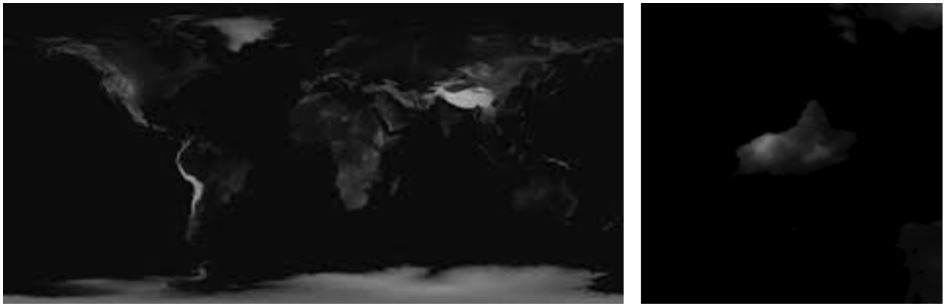
\includegraphics[width=0.9\textwidth]{images/modelowanie_terenu/przykladowe_heightmapy.jpg}
    \caption{Przykładowe mapy wysokościowe.}
\end{figure}

Kolejną istotną funkcjonalnością jest malowanie terenu drzewami. Umożliwia ona automatyczne umiejscowienie obiektów na
mapie w losowy sposób. Pozwala to szybko utworzyć realistyczne skupiska obiektów, takich jak las. Poniżej
został przedstawiony przykładowy rezultat. Wykorzystano do tego paczkę LowPoly Trees and Rocks dostępną w Unity
Assets Store.

\begin{figure}[h!]
    \centering
    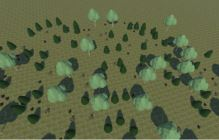
\includegraphics[width=0.5\textwidth]{images/modelowanie_terenu/drzewa.jpg}
    \caption{Widok na teren z drzewami.}
\end{figure}
